% Round 2 findings section

\subsection{Round 2}

\subsubsection{Performance}

%%%
% Discussion of performance
%%%

% Point spreads for two runs of blah

\begin{figure}
\center

\begin{subfigure}[b]{0.45\textwidth}
	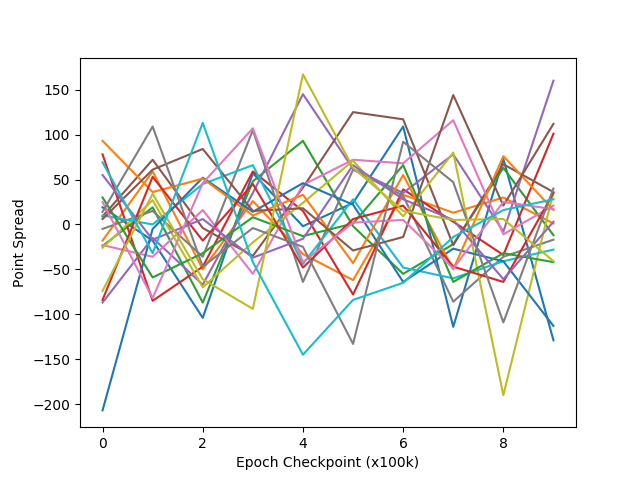
\includegraphics[width=\linewidth]{images/findings/round2/spreads_self-v-prev_winner.png}
	\caption{An agent plays against previous iterations of itself.}
	\label{fig:r2-spreads-winner-a}
\end{subfigure}
~
\begin{subfigure}[b]{0.45\textwidth}
	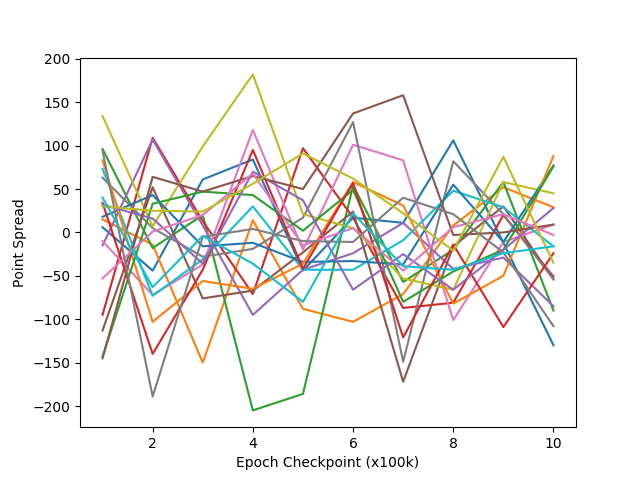
\includegraphics[width=\linewidth]{images/findings/round2/spreads_rand-v-fut_winner.png}
	\caption{A random agent plays against later, more learned agents.}
	\label{fig:r2-spreads-winner-b}
\end{subfigure}

\caption{
	Point spreads across twenty 9-game tournaments for an agent in the
	winners' bracket of Round 2.
	Note that since the winners' bracket uses an agent with prior training,
	the total epochs elapsed is one million more than displayed.
}
\label{fig:r2-spreads-winner}
\end{figure}


% Point spreads for two runs of blah

\begin{figure}
\center

\begin{subfigure}[b]{0.45\textwidth}
	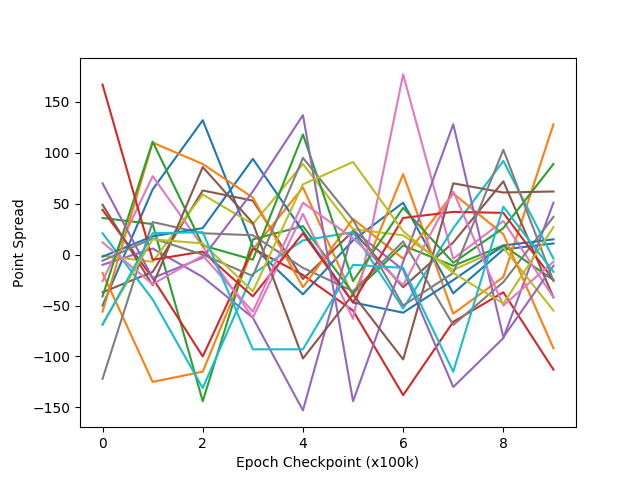
\includegraphics[width=\linewidth]{images/findings/round2/spreads_self-v-prev_loser.png}
	\caption{An agent plays against previous iterations of itself.}
	\label{fig:r2-spreads-loser-a}
\end{subfigure}
~
\begin{subfigure}[b]{0.45\textwidth}
	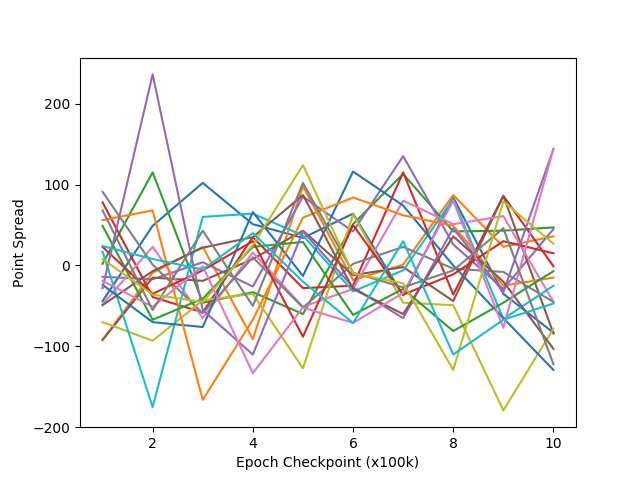
\includegraphics[width=\linewidth]{images/findings/round2/spreads_rand-v-fut_loser.png}
	\caption{A random agent plays against later, more learned agents.}
	\label{fig:r2-spreads-loser-b}
\end{subfigure}

\caption{
	Point spreads across mutliple 9-game tournamens of an agent in the
	losers' bracket of Round 2.
}
\label{fig:r2-spreads-loser}
\end{figure}




\subsubsection{Learning Process and Results}

%%%
% Discussion of what it learns and why that's interesting from a cribbage
% perspective
%%%


\begin{figure}
\center

	\begin{subfigure}[t]{0.22\textwidth}
		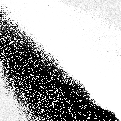
\includegraphics[width=\textwidth]{images/findings/round2/strats/winner/hand_max_min.png}
		\caption{\handmaxmin}
	\end{subfigure}
	~
	\begin{subfigure}[t]{0.22\textwidth}
		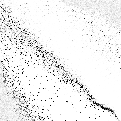
\includegraphics[width=\textwidth]{images/findings/round2/strats/winner/hand_max_avg.png}
		\caption{\handmaxavg}
	\end{subfigure}
	~
	\begin{subfigure}[t]{0.22\textwidth}
		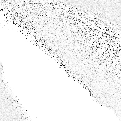
\includegraphics[width=\textwidth]{images/findings/round2/strats/winner/hand_max_med.png}
		\caption{\handmaxmed}
	\end{subfigure}
	~
	\begin{subfigure}[t]{0.22\textwidth}
		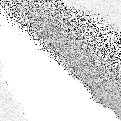
\includegraphics[width=\textwidth]{images/findings/round2/strats/winner/hand_max_poss.png}
		\caption{\handmaxposs}
	\end{subfigure}

	\begin{subfigure}[t]{0.22\textwidth}
		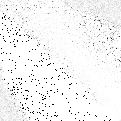
\includegraphics[width=\textwidth]{images/findings/round2/strats/winner/crib_min_avg.png}
		\caption{\cribminavg}
	\end{subfigure}
	~
	\begin{subfigure}[t]{0.22\textwidth}
		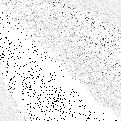
\includegraphics[width=\textwidth]{images/findings/round2/strats/winner/pegging_max_avg_gained.png}
		\caption{\peggingmaxavggained}
	\end{subfigure}
	~
	\begin{subfigure}[t]{0.22\textwidth}
		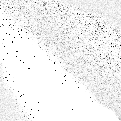
\includegraphics[width=\textwidth]{images/findings/round2/strats/winner/pegging_max_med_gained.png}
		\caption{\peggingmaxmedgained}
	\end{subfigure}
	~
	\begin{subfigure}[t]{0.22\textwidth}
		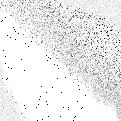
\includegraphics[width=\textwidth]{images/findings/round2/strats/winner/pegging_min_avg_given.png}
		\caption{\peggingminavggiven}
	\end{subfigure}

\caption{
	All final strategy strengths for an agent in the winners' bracket
	when playing as the dealer
	after training for one million games during Round 1
	and a further one million games during Round 2.
}
\label{fig:r2-strats-winner}
\end{figure}


%%%
Despite the lack of performance increase after another million games played by
both the winning and losing brackets,
there are still interesting trends to be spotted between the different brackets
of play.
%
The most notable is how quickly policies converge to a similar state.
%
While the strategy graphs for the less trained agents are less ``crisp''
in their appearance thanks to their smaller levels self-certainty,
the patterns of which policy to mainly follow at which times
are quick to form.
%
This is useful because it allows for the possibility of running future
experiments with fewer training epochs and thus in less time.
%
This in turn allows for a larger variety of methods to be tested to improve
the cribbage-playing agent.
%%%

%%%
Even more fascinating observations can be found from the strategy graphs
from the winner's bracket (see Figure~\ref{r2-strats-winner}).
%
By focusing on the \handmaxmin\ and \handmaxavg\ strategies in particular,
the sinusoidal wave along the diagonal can be observed extending further
back along the diagonal to earlier game positions,
albeit with smaller amplitude.
%
While not being of much use to the agent directly,
this is a useful observation from a cribbage player's perspective.
%
Since it is possible to infer the state-value function,
the implications of this wave are that earlier states are not crucial
predictors for future success.
%
Not only that,
but the agent has learned that changes in lead are likely and not necessarily
detrimental to the ability to win the game.
%%%

%%%
Care needs to be taken with this previous observation on the wave's amplitude
and it must be pointed out to be speculation on the part of the author.
%
It may be the case that with enough training the sine wave will be at full
amplitude in earlier positions.
%
A notable reason for the lack of clarity at the moment is the weight adjustment
mechanism for training.
%
The training system pre-supposes that the earlier positions are of less
importance in a game and adjusts them with a lower priority than later positions
in the game.
%
While two million games is speculated to be enough to counteract this
adjustment,
there is no evidence to either support or disprove this conclusion.
%%%


%%%
% Talking about loser's bracket and how it compares to winner's
%%%


\begin{figure}
\center

	\begin{subfigure}[t]{0.22\textwidth}
		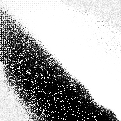
\includegraphics[width=\stratgraphwidth]{images/findings/round2/strats/loser/hand_max_min.png}
		\caption{\handmaxmin}
	\end{subfigure}
	~
	\begin{subfigure}[t]{0.22\textwidth}
		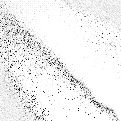
\includegraphics[width=\stratgraphwidth]{images/findings/round2/strats/loser/hand_max_avg.png}
		\caption{\handmaxavg}
	\end{subfigure}
	~
	\begin{subfigure}[t]{0.22\textwidth}
		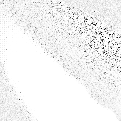
\includegraphics[width=\stratgraphwidth]{images/findings/round2/strats/loser/hand_max_med.png}
		\caption{\handmaxmed}
	\end{subfigure}
	~
	\begin{subfigure}[t]{0.22\textwidth}
		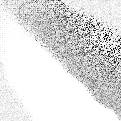
\includegraphics[width=\stratgraphwidth]{images/findings/round2/strats/loser/hand_max_poss.png}
		\caption{\handmaxposs}
	\end{subfigure}

	\begin{subfigure}[t]{0.22\textwidth}
		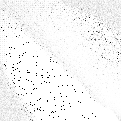
\includegraphics[width=\stratgraphwidth]{images/findings/round2/strats/loser/crib_min_avg.png}
		\caption{\cribminavg}
	\end{subfigure}
	~
	\begin{subfigure}[t]{0.22\textwidth}
		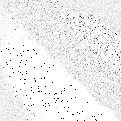
\includegraphics[width=\stratgraphwidth]{images/findings/round2/strats/loser/pegging_max_avg_gained.png}
		\caption{\peggingmaxavggained}
	\end{subfigure}
	~
	\begin{subfigure}[t]{0.22\textwidth}
		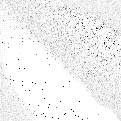
\includegraphics[width=\stratgraphwidth]{images/findings/round2/strats/loser/pegging_max_med_gained.png}
		\caption{\peggingmaxmedgained}
	\end{subfigure}
	~
	\begin{subfigure}[t]{0.22\textwidth}
		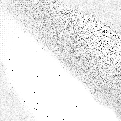
\includegraphics[width=\stratgraphwidth]{images/findings/round2/strats/loser/pegging_min_avg_given.png}
		\caption{\peggingminavggiven}
	\end{subfigure}

\caption{
	All final strategy strengths for an agent in the losers' bracket
	when playing as the dealer
	after training for one million games during Round 2.
}
\label{fig:r2-strats-loser}
\end{figure}


%%%
By comparing the winner's bracket strategy graphs to those of the loser's
bracket,
a vast degree of similarity can be found.
%
In both brackets,
the behavioral trends are learned.
%
However,
there does exist a small amount of difference between the two
in how quickly and surely each trend is learned.
%
The winner's bracket mostly reinforces its current weight choices
with the losing triangle becoming slightly gradiated.
% TODO: ^^^ gradiated (wrong) = to make something a gradient
Meanwhile,
in the loser's bracket,
the gradient applies more evenly to the entire range of strategies
across the winning-losing boundary.
%
Of additional note,
there are fewer spaces in which
strategies such as \cribminavg, \peggingmaxavggained, and \peggingminavggiven\ 
have been strengthened within the \handmaxmin\ \textit{block}.
%
This is a good indicator that,
although present,
there is less of a bias towards those strategies which are initially winners.
%%%


\begin{figure}
\center

	\begin{subfigure}[t]{0.22\textwidth}
		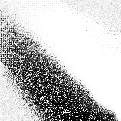
\includegraphics[width=\stratgraphwidth]{images/findings/round2/strats/random/hand_max_min.png}
		\caption{\handmaxmin}
	\end{subfigure}
	~
	\begin{subfigure}[t]{0.22\textwidth}
		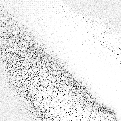
\includegraphics[width=\stratgraphwidth]{images/findings/round2/strats/random/hand_max_avg.png}
		\caption{\handmaxavg}
	\end{subfigure}
	~
	\begin{subfigure}[t]{0.22\textwidth}
		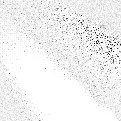
\includegraphics[width=\stratgraphwidth]{images/findings/round2/strats/random/hand_max_med.png}
		\caption{\handmaxmed}
	\end{subfigure}
	~
	\begin{subfigure}[t]{0.22\textwidth}
		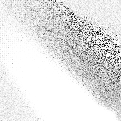
\includegraphics[width=\stratgraphwidth]{images/findings/round2/strats/random/hand_max_poss.png}
		\caption{\handmaxposs}
	\end{subfigure}

	\begin{subfigure}[t]{0.22\textwidth}
		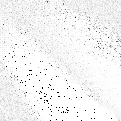
\includegraphics[width=\stratgraphwidth]{images/findings/round2/strats/random/crib_min_avg.png}
		\caption{\cribminavg}
	\end{subfigure}
	~
	\begin{subfigure}[t]{0.22\textwidth}
		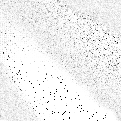
\includegraphics[width=\stratgraphwidth]{images/findings/round2/strats/random/pegging_max_avg_gained.png}
		\caption{\peggingmaxavggained}
	\end{subfigure}
	~
	\begin{subfigure}[t]{0.22\textwidth}
		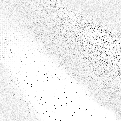
\includegraphics[width=\stratgraphwidth]{images/findings/round2/strats/random/pegging_max_med_gained.png}
		\caption{\peggingmaxmedgained}
	\end{subfigure}
	~
	\begin{subfigure}[t]{0.22\textwidth}
		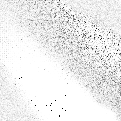
\includegraphics[width=\stratgraphwidth]{images/findings/round2/strats/random/pegging_min_avg_given.png}
		\caption{\peggingminavggiven}
	\end{subfigure}

\caption{
	All final strategy strengths for a learning agent
	after playing a completely random agent
	when playing as the pone
	after training for 350,000 games during Round 2.
}
\label{fig:r2-strats-random}
\end{figure}


%%%
% TODO: discuss random tourny's stuff
%%%

%%%
In analyzing the evolution of the \handmaxavg\ strategy in both the winner's
and loser's brackets,
it can clearly be seen that the general trend of behavior forms
quickly,
i.e. after the first half million games played.
%
Beyond that amount of games,
the agent learns to refine the strategy boundaries
but it can be said that there is little discovery being made.
%
This is useful because it allows for quicker training rounds to be played,
and thus more possible variations in training can be tried in the time given
with the goal of improving beyond random play.
%%%


% Figure for the flipbook of strategies over time

\begin{figure}
\center

	\begin{subfigure}[t]{0.2\textwidth}
	
\includegraphics[width=\textwidth]{images/findings/round2/flipbook/loser/checkpoint_000000.png}
	\caption{Starting Weights}
	\end{subfigure}
	~
	\begin{subfigure}[t]{0.2\textwidth}
	\includegraphics[width=\textwidth]{images/findings/round2/flipbook/loser/checkpoint_200000.png}
	\caption{After 200,000 games played}
	\end{subfigure}
	~
	\begin{subfigure}[t]{0.2\textwidth}
	\includegraphics[width=\textwidth]{images/findings/round2/flipbook/loser/checkpoint_400000.png}
	\caption{After 400,000 games played}
	\end{subfigure}

	\begin{subfigure}[t]{0.2\textwidth}
	\includegraphics[width=\textwidth]{images/findings/round2/flipbook/loser/checkpoint_600000.png}
	\caption{After 600,000 games played}
	\end{subfigure}
	~
	\begin{subfigure}[t]{0.2\textwidth}
	\includegraphics[width=\textwidth]{images/findings/round2/flipbook/loser/checkpoint_800000.png}
	\caption{After 800,000 games played}
	\end{subfigure}
	~
	\begin{subfigure}[t]{0.2\textwidth}
	\includegraphics[width=\textwidth]{images/findings/round2/flipbook/loser/checkpoint_999999.png}
	\caption{Final Weights}
	\end{subfigure}

\caption{
	Training weights representation for a losers' bracket agent's \handmaxavg\
	strategy when the agent is the dealer
	over the course of the one million games of Round 2.
}
\label{fig:r2-flip-loser}
\end{figure}


% Figure for the flipbook of strategies over time

\begin{figure}
\center

	\begin{subfigure}[b]{0.4\textwidth}
	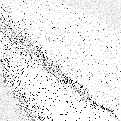
\includegraphics[width=\linewidth]{images/findings/round2/flipbook/winner/checkpoint_000000.png}
	\caption{Starting Weights}
	\end{subfigure}
	~
	\begin{subfigure}[b]{0.4\textwidth}
	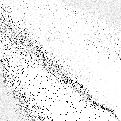
\includegraphics[width=\linewidth]{images/findings/round2/flipbook/winner/checkpoint_200000.png}
	\caption{After 200,000 games played}
	\end{subfigure}

	\begin{subfigure}[b]{0.4\textwidth}
	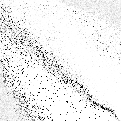
\includegraphics[width=\linewidth]{images/findings/round2/flipbook/winner/checkpoint_400000.png}
	\caption{After 400,000 games played}
	\end{subfigure}
	~
	\begin{subfigure}[b]{0.4\textwidth}
	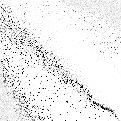
\includegraphics[width=\linewidth]{images/findings/round2/flipbook/winner/checkpoint_600000.png}
	\caption{After 600,000 games played}
	\end{subfigure}

	\begin{subfigure}[b]{0.4\textwidth}
	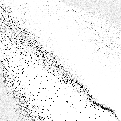
\includegraphics[width=\linewidth]{images/findings/round2/flipbook/winner/checkpoint_800000.png}
	\caption{After 800,000 games played}
	\end{subfigure}
	~
	\begin{subfigure}[b]{0.4\textwidth}
	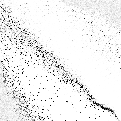
\includegraphics[width=\linewidth]{images/findings/round2/flipbook/winner/checkpoint_999999.png}
	\caption{Final Weights}
	\end{subfigure}

\caption{
	Training weights representation for a winner bracket agent's \handmaxavg\
	strategy when the agent is the dealer
	over the course of the one million games of Round 2.
	Note that the starting weights are carried over from Round 1,
	so the total training epochs to reach each position is actually
	one million higher than expressed.
}
\label{fig:r2-flip-winner}
\end{figure}


% Figure for the flipbook of strategies over time

\begin{figure}
\center

	\begin{subfigure}[b]{0.4\textwidth}
	
\includegraphics[width=\linewidth]{images/findings/round2/flipbook/random/checkpoint_000000.png}
	\caption{Starting Weights}
	\end{subfigure}
	~
	\begin{subfigure}[b]{0.4\textwidth}
	\includegraphics[width=\linewidth]{images/findings/round2/flipbook/random/checkpoint_200000.png}
	\caption{After 200,000 games played}
	\end{subfigure}

	\begin{subfigure}[b]{0.4\textwidth}
	\includegraphics[width=\linewidth]{images/findings/round2/flipbook/random/checkpoint_400000.png}
	\caption{After 400,000 games played}
	\end{subfigure}
	~
	\begin{subfigure}[b]{0.4\textwidth}
	\includegraphics[width=\linewidth]{images/findings/round2/flipbook/random/checkpoint_600000.png}
	\caption{After 600,000 games played}
	\end{subfigure}

	\begin{subfigure}[b]{0.4\textwidth}
	\includegraphics[width=\linewidth]{images/findings/round2/flipbook/random/checkpoint_800000.png}
	\caption{After 800,000 games played}
	\end{subfigure}
	~
	\begin{subfigure}[b]{0.4\textwidth}
	\includegraphics[width=\linewidth]{images/findings/round2/flipbook/random/checkpoint_999999.png}
	\caption{Final Weights}
	\end{subfigure}

\caption{
	Training weights representation for a winner bracket agent's \handmaxavg\
	strategy when the agent is the dealer
	over the course of the one million games of Round 2.
}
\label{fig:r2-flip-random}
\end{figure}



